\setcounter{page}{2}
\section{Въведение}
Целта на настоящата дипломна работа е да представи моделите и резултатите получени по време на работата ми \sout{през изминалата година с.(няма смисъл да ме споменаваш тук - по-важно е тематиката да е пояснена добре)}. Крайната цел е да се моделира процесът на кристален растеж при различни условия и да се развие разбирането как експерименталните условия влияят на кинетиката на процеса и на крайната структура на кристала. В този контекст ще бъде направен и преглед на част от публикуваните експериментални данни с цел валидиране на моделите и подобряване на разбирането на тези резултати с разработените нови инструменти.
\textbf{Тук ако ти се вижда смислено, по-добре да кажеш нещо за това, че работата е част от една траектория, която сочи надалеч или може би дори се надяваш, че това си личи ..дори ако ти идва отвътре - каже, че това е фрагмент от дисертацията ти! :)}

\sout{В най-общ смисъл настоящият труд може да бъде разделен на две основни части - моделиране на зависимостта на степента на превръщане $\alpha$ от времето (макроскопско моделиране) и моделиране на т.нар. ,,step-flow growth``  (моделиране на микроскопския механизъм). Преди това е нужно да бъде направено кратко въведение в представите за кристализацията като процес, разработени през късните години на миналия век.}
Тук трябва да подходим по-директно:
В първата част е представен развит напоследък от нас модел на кристален растеж в условията на изчерпащо се пресищане (движещата сила на процеса на кристализация), като в центъра на разглежданията е диференциално у-ние за степента на превръщане, получено от израз за норналаната скорост ба растеж.
Това придвижване на кристалната стена в неподредената фаза може да бъде и резултантно - получено от общото действие на много тангенциални .. Във втората част 

\subsection{Критични явления и фазови преходи може да се обърне словореда!}
Кристализацията е от т.нар. ,,фазови преходи`` и по-точно е фазов преход от \textit{първи род}. Класификацията на фазови преходи от \textit{първи} и \textit{втори} род е дадена от Пол Еренфест \cite{Jaeger1998} \cite{atkinspaula2008} и представлява важен инструмент за разбирането на промените, които настъпват по време на процеса.

\begin{definition}{Класификация на Еренфест на фазовите преходи}{ehrenfest}
	По време на фазов преход от \textbf{n}-ти род, \textbf{n}-тата производна на вътрешната енергия ($\frac{\partial^n U}{\partial X^n}$) \textbf{U} по някоя термодинамична величина (\textbf{X}) търпи скок в критичната точка $\boldsymbol{X_c}$. \textbf{X} може да бъде температура (\textbf{T}), налягане (\textbf{p}), обем (\textbf{V}) и т.н.
\end{definition}

\noindent Физически важни са фазовите преходи от \textit{първи} и \textit{втори} род:

По време на фазов преход от \textit{първи род} \textbf{в точката на прехода} съществуват едновременно и двете фази - течност/газ, течност/твърдо и т.н. ПроцесЪТ е свързан и с т.нар. ,,латентна ТОПЛИНА енергия``, което означава че системата приема или отдава фиксирано количество енергия (най-често топлина) за единица маса или обем. Системата тогава остава при постоянна температура по време на прехода като цялата отдадена/погълната енергия отива за формирането на новата фаза.

Фазовите преходи от \textit{втори род} се характеризират с плавна ($C^1$-непрекъсната) промяна на вътрешната енергия. Те обикновено са свързани със скок в т.нар. ,,възприемчивости`` на системата - магнитна възприемчивост, топлинен капацитет и други. Няма фазови граници между отделните фази и няма латентна топлина. Пример за такъв фазов преход е нагряването на магнит до неговата точка на Кюри. Характеристична за тези фазови преходи е безкрайната корелационна дължина в критичната точка. Прост модел за изследването на такива фазови преходи е моделът на Изинг за свойствата на феромагнитите в размерности на пространството по-големи от 1, който може да се приложи и за изследването на магнитните свойства на кристалите. Въпреки че тези фазови преходи са изключително интересни от физична и математическа гледна точка, те няма да бъдат предмет на настоящата работа.

\subsection{Термодинамика на кристализацията}
\label{sub:thermodynamics}
Имайки предвид \autoref{def:ehrenfest} естествен първи подход за моделиране на кристализацията е да използваме термодинамиката на многокомпонентните системи.

\begin{definition}{Химичен или химически??? потенциал}{chempot}
    Химичният потенциал е промяната във вътрешната (свободната) енергия, която би настъпила при промяна на броя частици от даден химичен вид/фаза в системата. Най-често се отбелязва с $\mu$.
	\begin{equation}
		\label{eq:chempot}
		\mu_i = \left(\frac{\partial U}{\partial N_i}\right)_{S, V, N_{i \ne j}}
	\end{equation}
	Където индексът $S, V, N_{i \ne j}$ означава, че ентропията, обемът и броят други частици в системата са постоянни при изчисляване на производната.
\end{definition}

\noindent Следва да се отбележи, че абсолютната стойност на химичния потенциал не може да бъде измерена на практика. Нейната стойност (промяната ѝ) спрямо тази при определени референтни условия обаче може лесно да бъде получена експериментално. Затова и в литературата най-често се откриват табулирани стойностите на $\Delta \mu$ измерени по отношение на стандартни термодинамични условия ($T \approx 273~K, p \approx 1~atm$) \cite{IvanMarkovCGB}\cite{atkinspaula2008}.

\begin{result}{ ЧИЙ??? Условие за фазово/химично равновесие}{equil_cond}
	\[\sum\limits_i \nu_i\Delta \mu_i  = 0\]
	Където $\nu_i$ е т.нар. ,,стехиометричен коефициент``. За фазови преходи най-често $\nu_i = 1$ (една частица от фаза $\alpha$ преминава във фаза $\beta$).
\end{result}

\noindent Тогава можем директно да приложим уравнението за идеален разтвор към течната фаза:

\begin{align}
	\Delta \mu_{i} & = \left( \mu_{i}^\circ + RT\ln{c_i} \right) - \left( \mu_{i}^\circ + RT\ln{c_{i}^{eq}} \right) \nonumber \\
	\Delta \mu_{i} & = RT\ln{\frac{c_i}{c_{i}^{eq}}} \nonumber                                                                \\
	\Delta \mu_{i} & = RT\ln{\sigma} \label{eq:thermodynamic_force}                                                           
\end{align}

\noindent Където дефинираме:
\begin{equation}
	\label{eq:abs_supersat}
	\sigma \coloneqq \frac{c_{i}}{c_{i}^{eq}}
\end{equation}
Да бъде т.нар. ,,абсолютно пресищане``. Тогава \autoref{eq:thermodynamic_force}, заедно с условието за равновесие \autoref{res:equil_cond} ни дава термодинамичната движеща сила.

Кристализационният процес, от термодинамична гледна точка, е обусловен от абсолютното пресищане $\sigma > 1$. В граничния случай на равновесие $\sigma = 1$ ($c_{i}  = c_{i}^{eq}$). Този резултат е интуитивно смислен - ,,излишъкът``от частици в течната фаза преминават в кристалната \cite{IvanMarkovCGB}

Има много начини да бъде постигнато пресищане $\sigma > 1$ от експериментална гледна точка. Най-честият начин е наситен ($\sigma = 1$) за дадена температура разтвор да бъде охладен рязко, като други възможности са електрохимично да се промени разтворимостта, добавяне на друг електролит и разрушаване на солватната обвивка и т.н. 

Въпреки че термодинамичният модел е много лесен за получаване и разбиране, той единствено може да покаже коя е термодинамичната движеща сила, без да дава отговор на следните практически важни въпроси:
\begin{enumerate}
	\item Как започва кристалният растеж?
	\item Как скоростта на кристализация (трансформация) зависи от пресищането?
	\item Кристалите имат симетрия, която се репродуцира на всички мащаби. Какви са механизмите зад това?
	\item Как крайният размер на фазите влияе на растежа?
	\item \textbf{Какъв е микроскопският механизъм на процеса?}
\end{enumerate}

В следващите параграфи на това въведение ще бъде направен преглед на трудовете на Странски, Каишев, Кръстанов, Марков, Бъртон и др., който ще очертае основите на механизма възпроизводимият кристален растеж. Това ще послужи и като основа за моделите, които ще разработим.

\subsection{Микроскопски представи за кристалния растеж}
\label{sub:microscopic_growth}
Както беше споменато, горните разглеждания са чисто макроскопски и не взимат предвид реалното адсорбиране-десорбиране на градивните единици на кристалите - атоми, молекули, йони. Ще започнем прегледа като въведем някои общи дефиниции и нотация:
\begin{figure}[htbp]
	\centering
	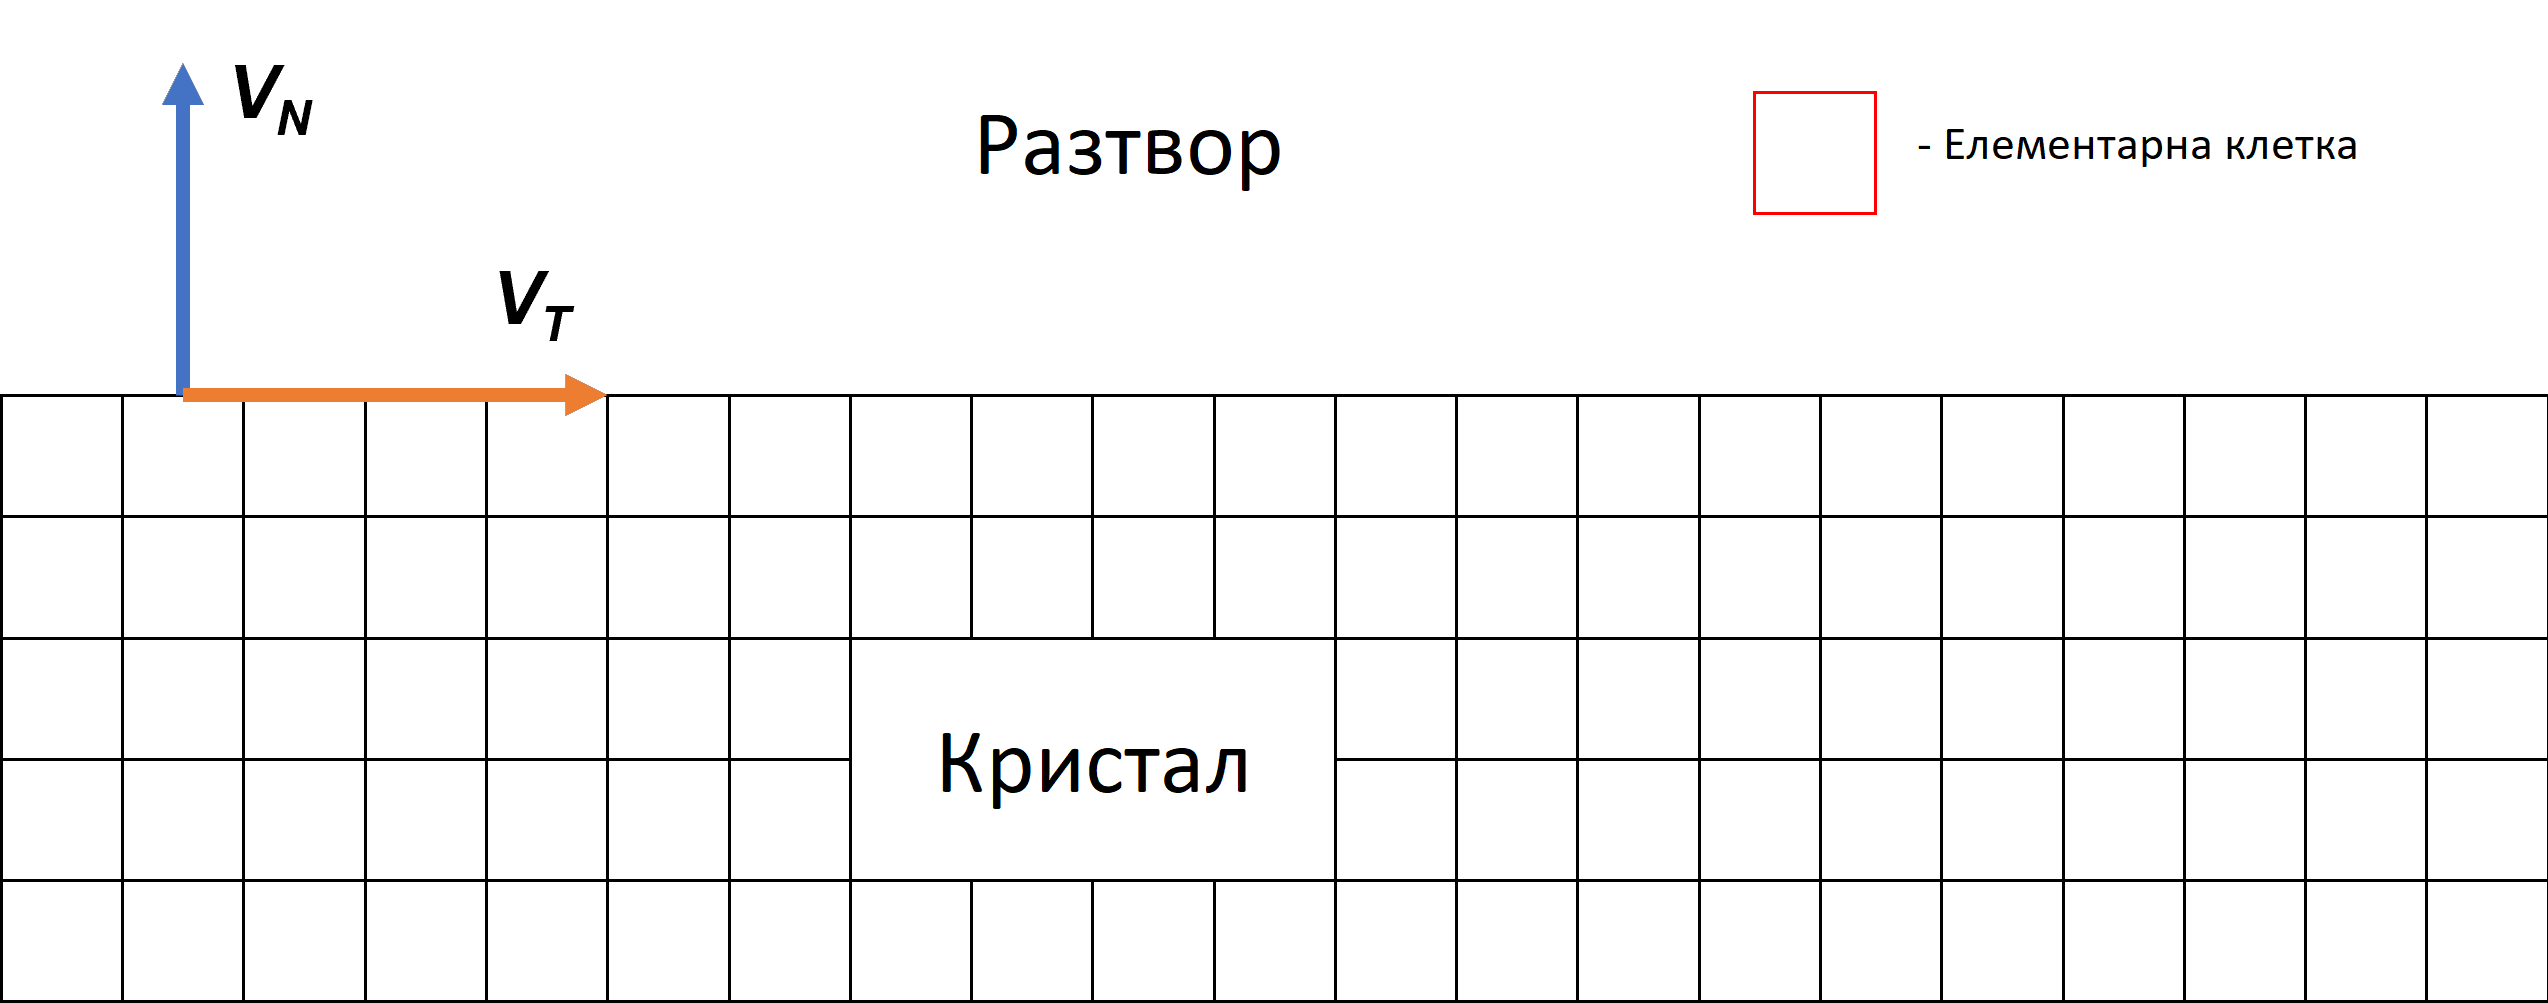
\includegraphics[width=\textwidth]{crystal_coord_system.png}
	\caption{Схематично представяне на растящ в разтвор кристал}
\end{figure}

\noindent Ще означаваме с $\boldsymbol{V_{N}}$ външната нормала към кристалната повърхност, а с $\boldsymbol{V_{T}}$ - единичния вектор тангенциален към повърхността. Също така ще предполагаме, че безкраен кристал без дефекти е изграден изцяло от т.нар. \textbf{елементарни клетки}, регулярно транслирани в посоките на пространството, така че да се получи плътна опаковка.

\begin{definition}{Елементарна клетка}{unit_cell}
    Елементарната клетка е най-малката структура от атоми, йони или молекули, която напълно отразява структурата на целия кристал. Целият кристал може да бъде изцяло изграден чрез транслиране на елементарната клетка по посока на главните координатни оси.
\end{definition}

Съществуването на повтаряща се структура като елементарната клетка, чиято група на симетрия се възпроизвежда на всички мащаби, дава една посоките за отговор на част от въпросите поставени в \autoref{sub:thermodynamics}. Кинетичният механизъм обаче остава все още неясен. За краткост като синоним на ,,елементарна клетка`` ще използваме понятието ,,градивна единица``.

\begin{figure}[ht]
	\centering
	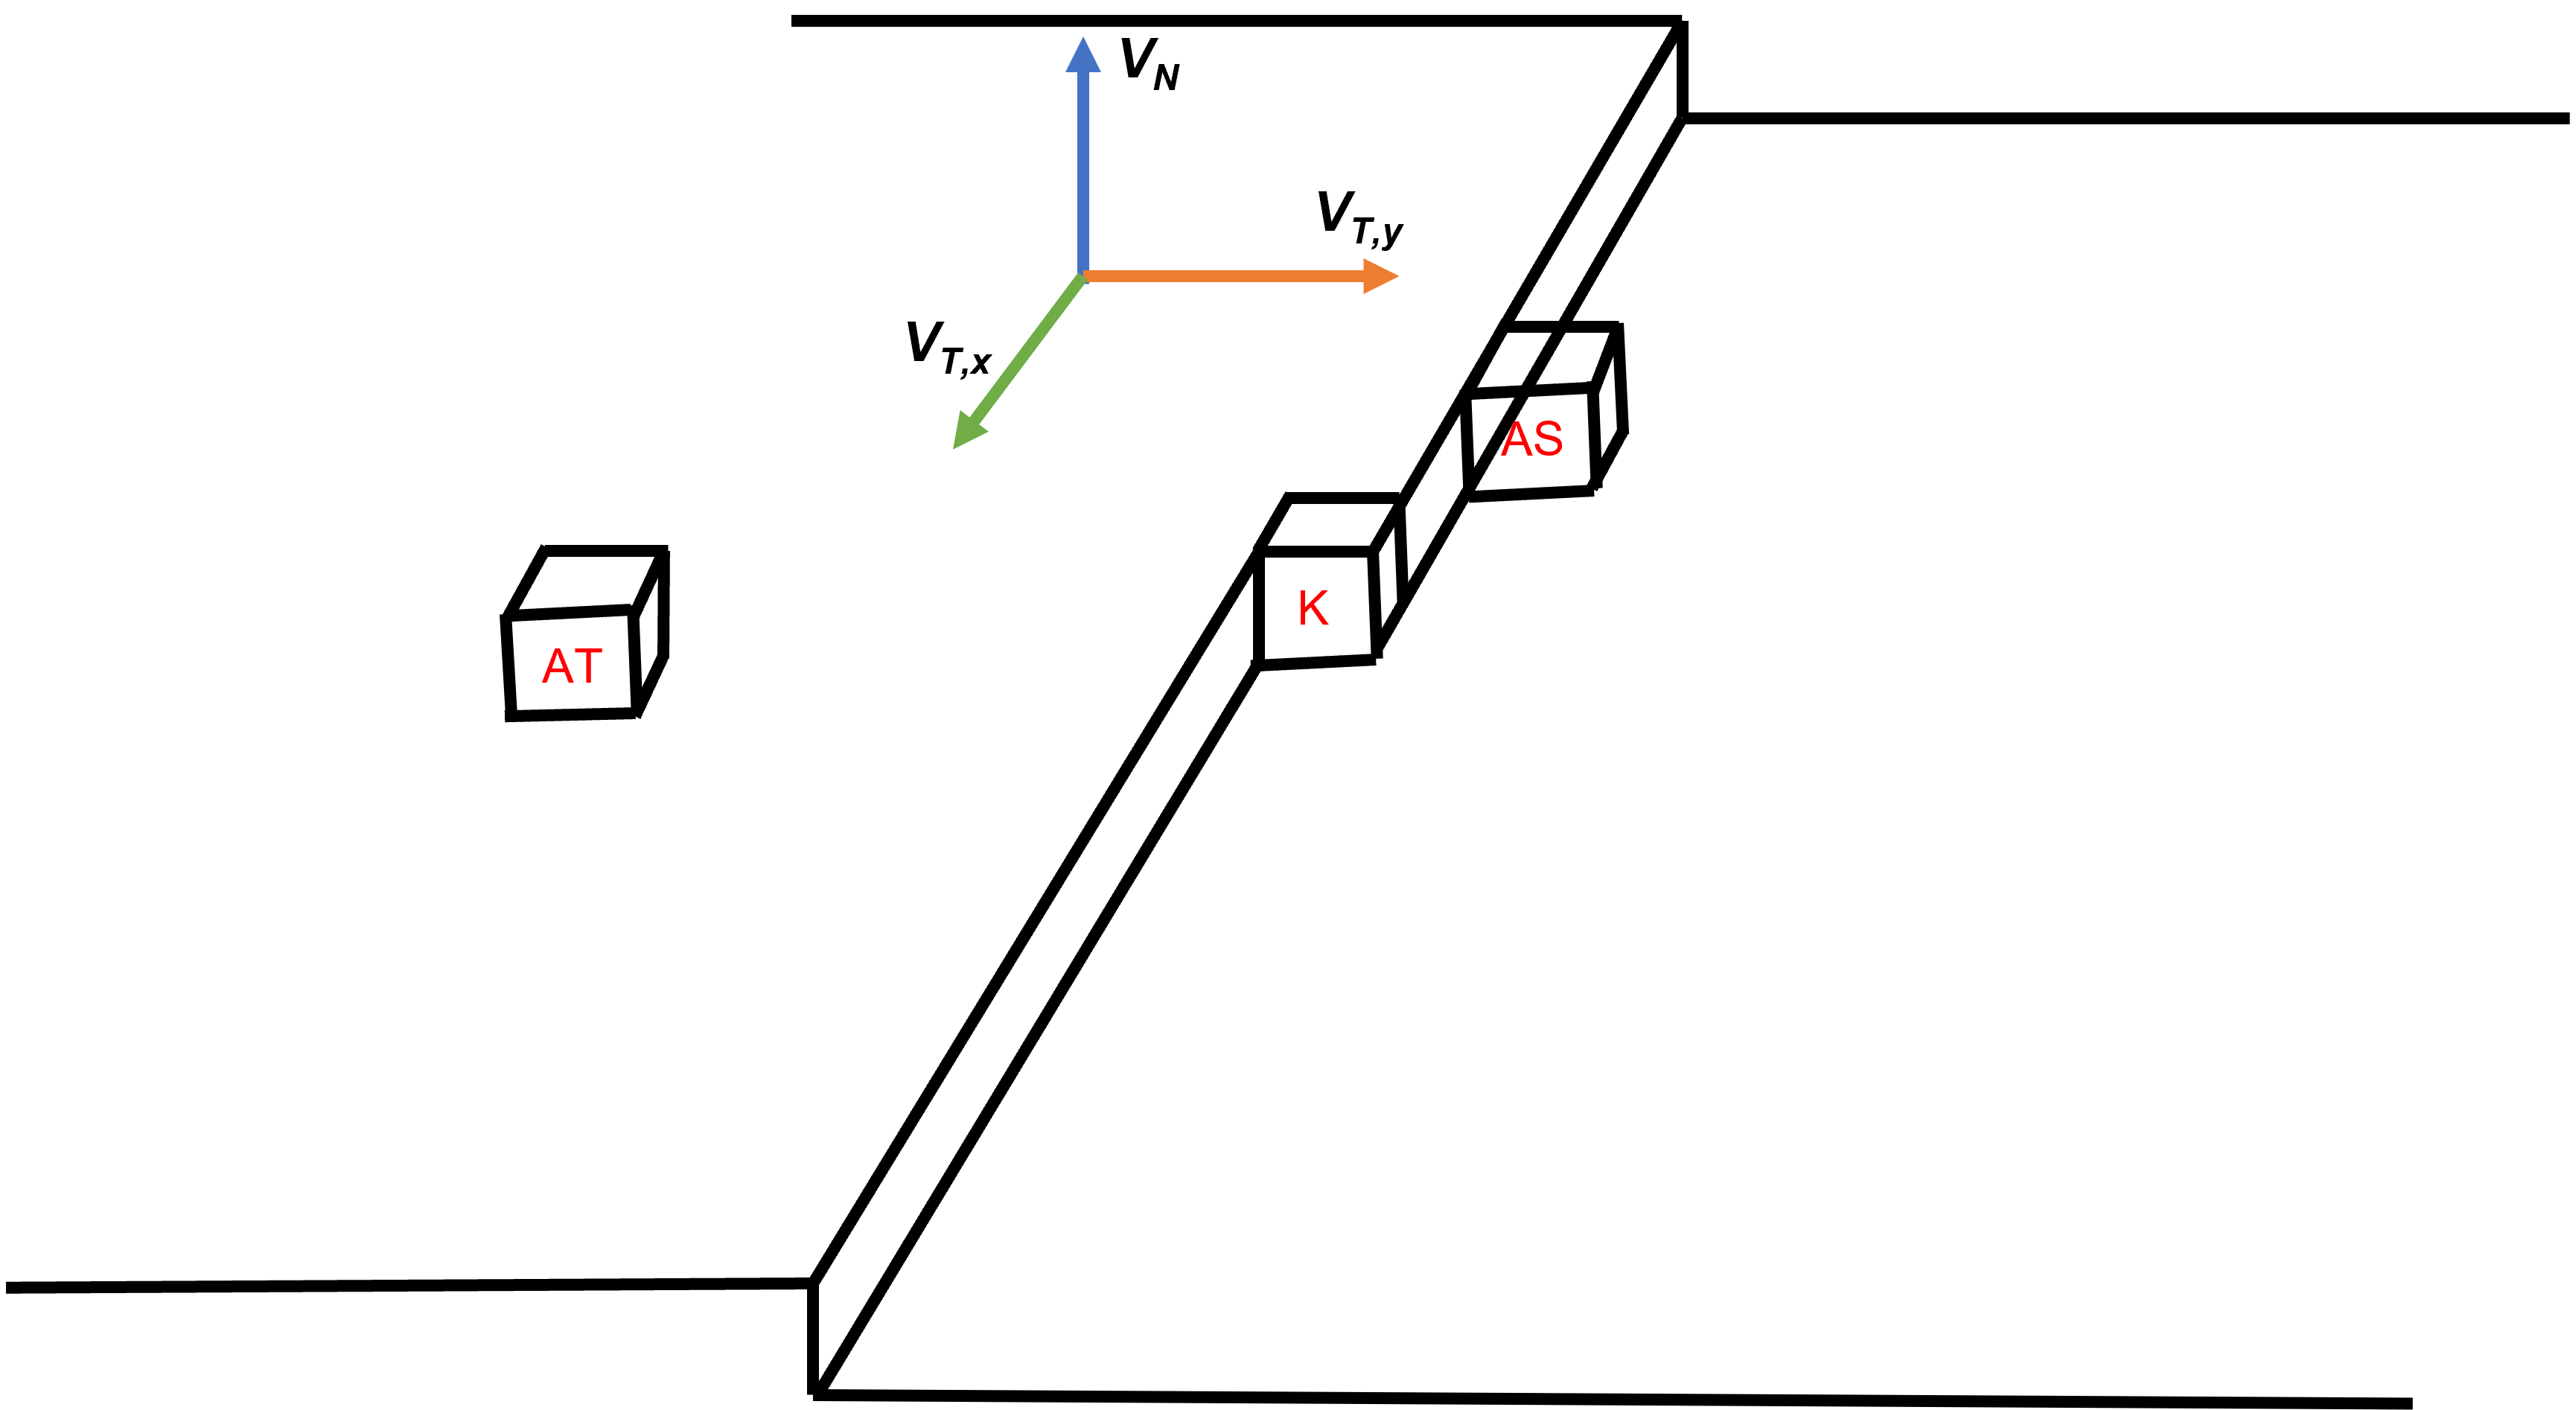
\includegraphics[width=\textwidth]{kink_pos.png}
	\caption{Позиции на растящата кристална повърхност:  \textcolor{red}{K} - кинк-позиция, \textcolor{red}{AT} - атом адсорбиран на терасата, \textcolor{red}{AS} - атом адсорбиран на стъпалото. }
	\label{fig:atoms_on_surface}
\end{figure}

Основите на съвременната кинетична теория поставят Странски и Косел независимо един от друг през 1927~г. \cite{Stranski1928}\cite{Kossel1927} като въвеждат идеята за работа, необходима за отделяне на градивна единица от т.нар. позиция на ,,полу-кристал`` или ,,кинк-позиция``. Тези представи свързват именно морфологията на растящата кристална повърхност с механизма на растеж.

От представените на  \autoref{fig:atoms_on_surface} позиции е ясно, че най-здраво свързани са атомите в обема на кристала. Новите адатоми обаче могат да се свържат само към повърхността му. В позиция \textcolor{red}{К} градивната частица има същият брой връзки като в обемния кристал, въпреки че са само ,,половин-връзки``, докато в позиции \textcolor{red}{AT} и \textcolor{red}{AS} e по-слабо свързана. Като следствие от това, свързването към кинк-позиция води до най-голямо понижаване на вътрешната енергия на свързващата се градивна единица и най-много отделена латентна топлина, и съответно е термодинамично най-устойчивата позиция. Това може да бъде илюстрирано още по-добре ако бъде разгледана и една странична (едномерна) проекция на растящата кристална повърхност, където представянето на кинк-позицията като най-енергийно изгодната такава става очевидно.

Такава проекция е представена на \autoref{fig:side_proj_kink}. От нея става освен това очевиден и друг централен факт - свързването към кинк-позиция води до формирането на нов кинк.
Това е основното ,,зъбно колело`` в механизма на възпроизводимия кристален растеж представен от Странски, Косел и Каишев \cite{Stranski1928} \cite{Kossel1927} \cite{StranskiKaischew1931}.
\begin{figure}[H]
	\centering
	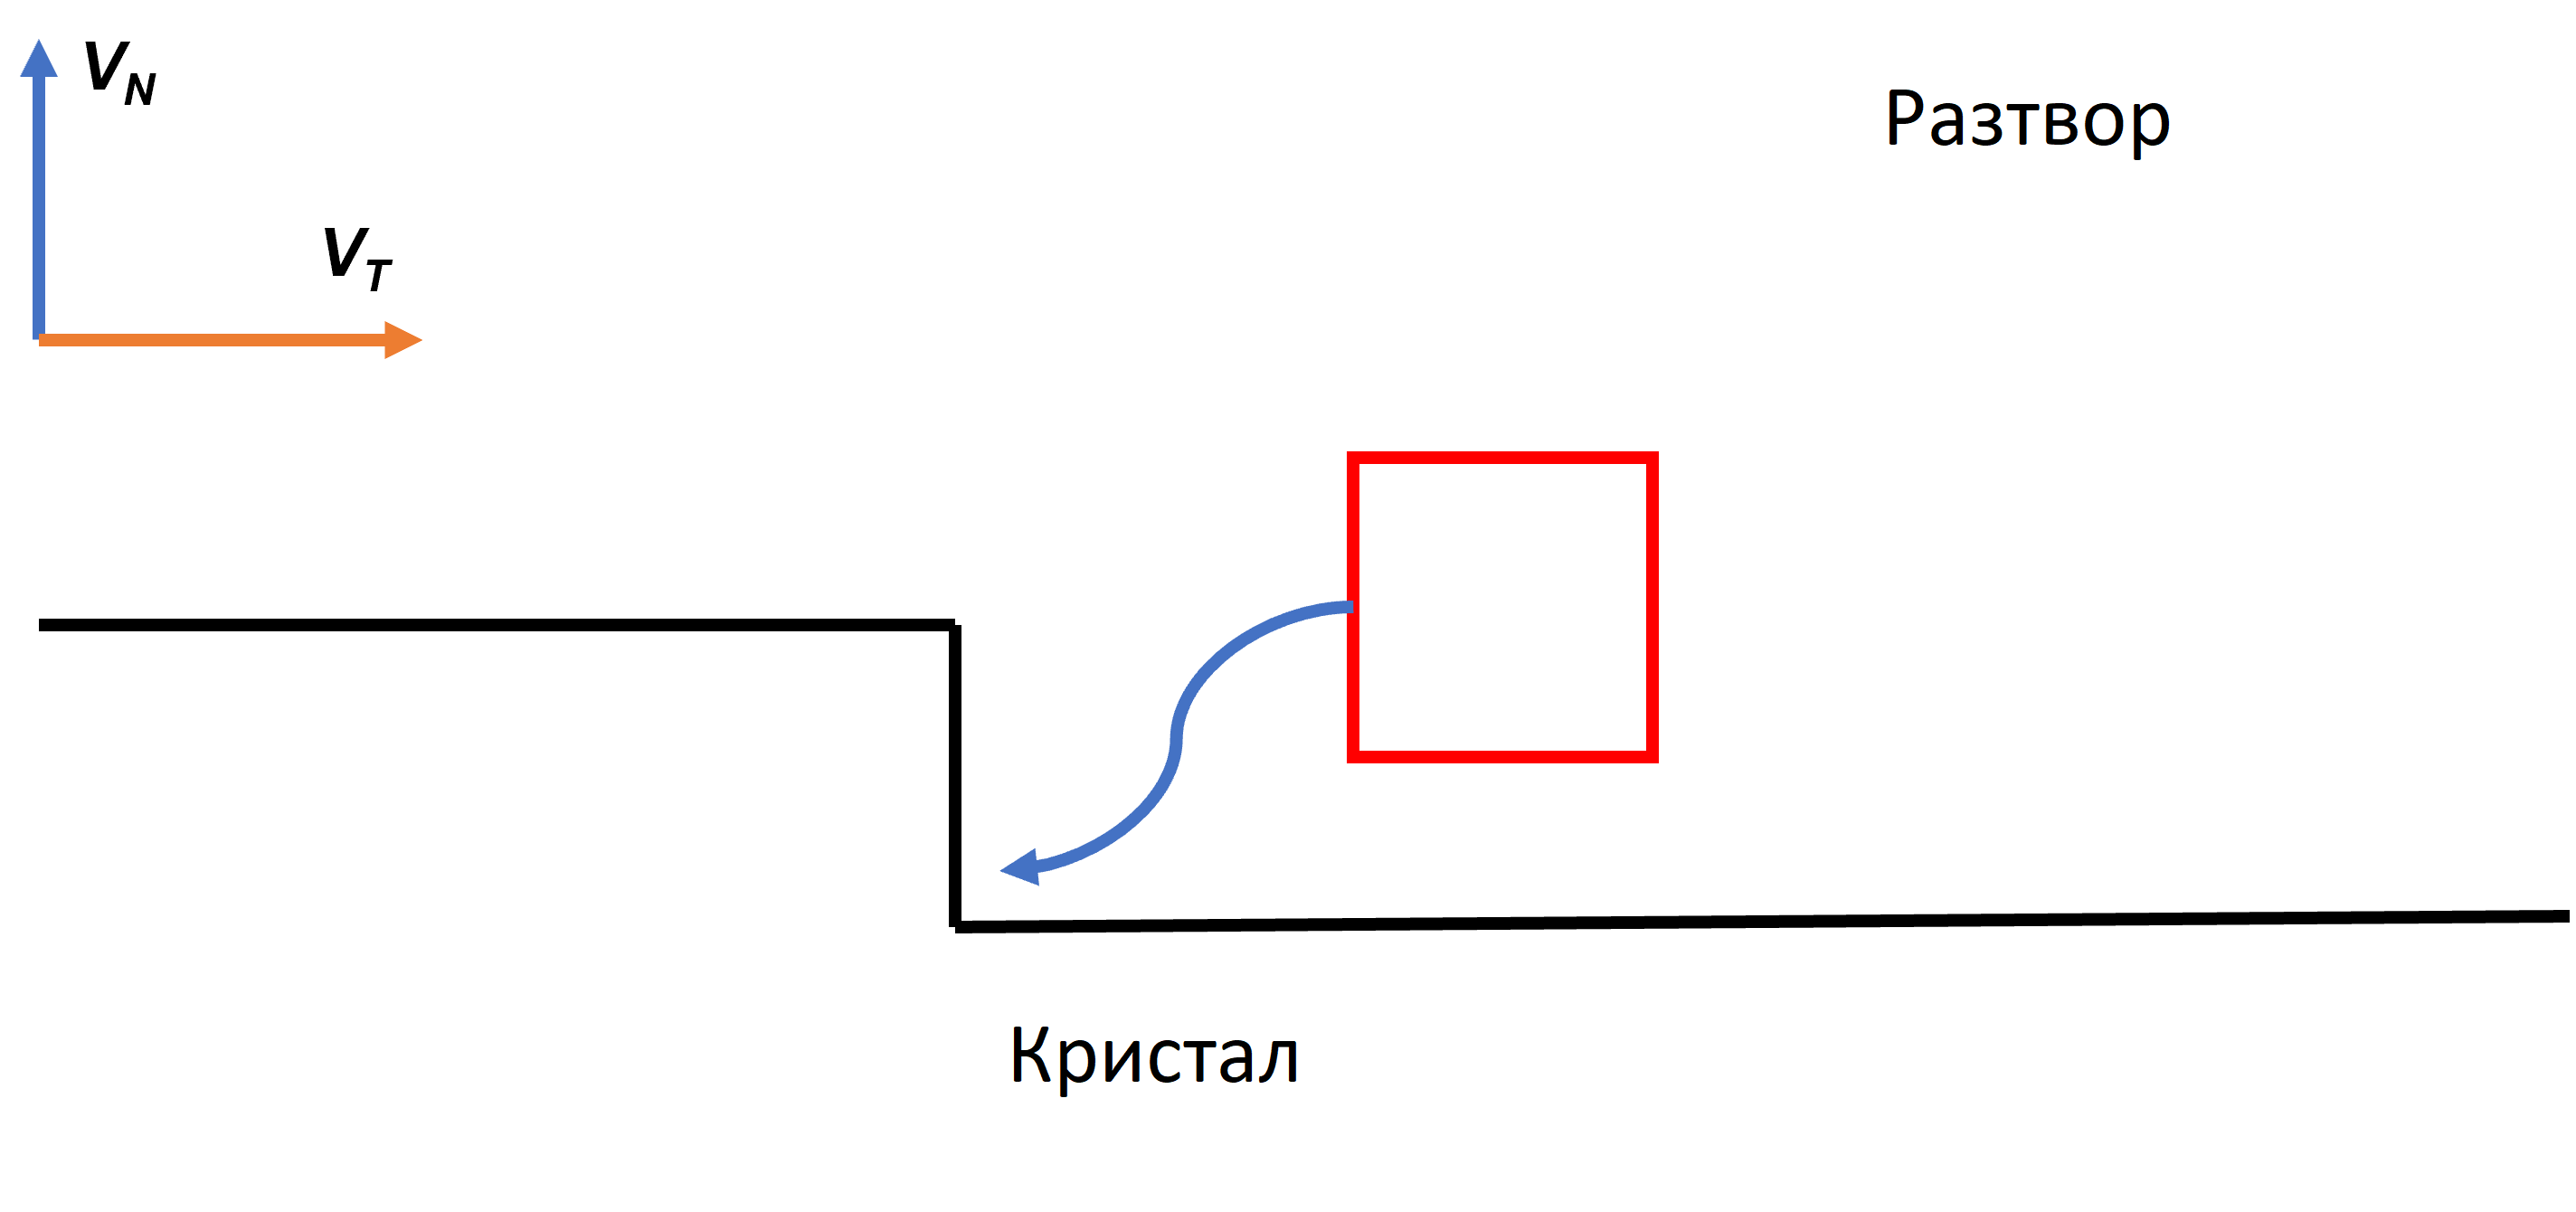
\includegraphics[width=\textwidth]{side_proj_kink.png}
	\caption{Странична (1D) проекция на кристалната повърхност}
	\label{fig:side_proj_kink}
\end{figure}

Идеята за кинк-позицията, комбинирана с тази за елементарната клетка като основна градивна единица, носеща цялата информация за кристала дава обяснение на въпроса за кристалната симетрия. Още повече, става ясно че растежът е послоен - новите градивни единици се свързват към кинк-позиции, докато настоящият слой от кристалната стена е изцяло изграден. Така ,,тангенциалният растеж`` (по посока на  $\boldsymbol{V_{T,x}}$ и $\boldsymbol{V_{T,y}}$) обуславя ,,нормалния`` (по посока на $\boldsymbol{V_{N}}$) и в крайна сметка - напредването на кристалната стена в разтвора.

От описаната картина обаче се вижда и недостатък на този механизъм - тъй като кристалите са крайни обекти, в даден момент всички кинкове са изчерпани. Затова към тези представи е необходимо да се добави и идеята за комплементарни събития на свързването към кинк-позиция. Природата на тези комплементарни събития може да е доста разнообразна - агрегация, зародишообразуване и т.н., но могат да бъдат обединени под общото название за ,,кинк-образуващи`` събития.
Процесът на образуване като правило може да е доста сложен - особено в случая на тримерен растеж, тъй като свързването на единствена градивна единица към атомно гладка кристална повърхност не води до образуване на кинк. Това ясно се вижда при позиция \textcolor{red}{AT} на \autoref{fig:atoms_on_surface}.

През 1931~г. Каишев и Странски доказват т.нар. теорема на \textit{Каишев-Странски-Волф} - градивни единици, които са свързани по-слабо от такава в кинк-позиция са ,,преходни`` - те не принадлежат към равновесната форма на кристала. Въпреки това, те могат да бъдат важна част от кинетиката на процеса (напр. като част от кинк-образуващи събития). \cite{StranskiKaischew1931}\cite{Yamamoto1988}

Комбинацията от тези идеи е довела до т.нар. ,,Terrace-Ledge-Kink`` (TLK) модел на кристалния растеж, който е бил предпоставка за основополагащия кинетичен модел на Бъртон-Кабрера-Франк (BCF), следствие от който ще бъде основа за нашите модели. \cite{BCF1951}\cite{Chernov2004}

През 30-те години на XX~век започва и паралелно развитие на модели за целите на металургията и описание на фазовите преходи, които могат да се наблюдават там. Ранните успехи на тази област до голяма степен се дължат на на Джонсън, Мел, Аврами и Колмогоров (JMAK) \cite{Mehl1939} \cite{Lambrigger1998}. Те успяват да изведат прост аналитичен модел за изследване на данни за т.нар. степен на превръщане $\alpha$ (интуитивно, какъв процент от кристализацията е приключила в даден момент от процеса).

\begin{result}{JMAKn}{jmak}
    Ще означаваме с JMAKn семейството от криви:
    \begin{equation}
        \label{eq:jmak}
        \alpha(t) = 1 - e^{ - k t^n }
    \end{equation}
    Където $\alpha$ - степен на превръщане, $n = D$ (D е броят на пространствените измерения, в които растежният процес се случва - 1, 2, 3) или $n = D+1$ (ако се наблюдава допълнително зародишообразуване), а $k$ - ,,материална константа`` (носеща температурната зависимост на процеса).
\end{result}

%% TODO: Maybe add graphs for different values of n in JMAKn

JMAKn е придобил широка популярност като основен инструмент за ,,фитване`` на данни със сигмоидна форма от кристален растеж при разнообразни условия. Нещо повече - простотата на този модел го е направила толкова популярен, че до голяма степен условията и предположенията, при които е изведен са ,,забравени``. Могат да бъдат намерени публикувани експериментални данни, спрямо които е направена параметрична идентификация за $n$ в JMAKn и получените стойности не са целочислени (напр. $n = 1.725$) \cite{Min2005}. Това е довело до дискусии в областта дали кристалният растеж може да се случва в ,,брой`` пространствени измерения, който не е цяло число (т.нар. фрактален кристал), без първо да се вземе под внимание дали предпоставките, за които JMAKn е изведен са валидни за конкретните експериментални условия. Нецелите стойности на $n$ водят и до размерности на $k$, които трудно могат да бъдат обяснени (напр. какво би значело $[k]=T^{-1.725}$. Така възниква ситуация, в която се правят опити експериментът да бъде напаснат към и да обясни модела, а не обратното.

Съществуват и различни алтернативи на JMAKn, като най-често се използва моделът на Ричардс - и по-точно неговите частни случаи - моделите на Гомперц и Ферхюлст. Тези сигмоидни криви при параметрични идентификация дават също малки остатъчни дисперсии, но пък са изведени за популационен растеж. Това прави също трудна физическата интерпретация на получените стойности.

Всички тези недостатъци на настоящите инструменти за моделиране на времевата еволюция на степента на превръщане $\alpha$ очертават нуждата за нов модел, изведен от първи принципи за изотермична кристализация от разтвор. Това ще бъде и целта на следващите параграфи.